\documentclass{beamer}

\usepackage[T2A]{fontenc}
\usepackage[utf8x]{inputenc}
\usepackage[english,bulgarian]{babel}
\usepackage{multirow}

\mode<presentation> {
	\usetheme{Berlin}
}

%\usebackgroundtemplate {
%	\includegraphics[width=370px, height=270px, trim=0 0 0 -80px]{background}
%}

\graphicspath{{../images/}}

\title{Разширени графични възможности и вероятностни разпределения}
\subtitle{Статистическа обработка на данни с R}

\author{Пламен Петров и Тодор Балабанов}

\date{1.VI.2020}

\institute[ЦО и ИИКТ към БАН] {
	Център за обучение \\
	Институт по информационни и комуникационни технологии \\ 
	Българската академия на науките \\
	\medskip
	\textit{p.petrov@iit.bas.bg todorb@iinf.bas.bg}
}

\addtobeamertemplate{navigation symbols}{}{
	\usebeamerfont{footline}
	\usebeamercolor[fg]{footline}
	\hspace{1em}
	\insertframenumber/\inserttotalframenumber
}

\begin{document}

\begin{frame}
	\titlepage
\end{frame}

\section*{Теми}
\begin{frame}[shrink]
	\frametitle{Съдържание}
	\tableofcontents
\end{frame}

\section{Разширени графични възможности}

\begin{frame}
\center \huge{Разширени графични възможности}
\end{frame}

\subsection{Хистограми и плътности}

\begin{frame}
\frametitle{Визуализация по форма на случайни величини}
\begin{block}{Хистограма и плътност}
library( ggplot2 )

ggplot(data=diamonds) + geom\_histogram(aes(x=carat))

ggplot(data=diamonds) + geom\_density(aes(x=carat),fill=$"$grey50$"$)
\end{block}
\end{frame}

\begin{frame}
\frametitle{Хистограма при 30 групи}
\begin{figure}[]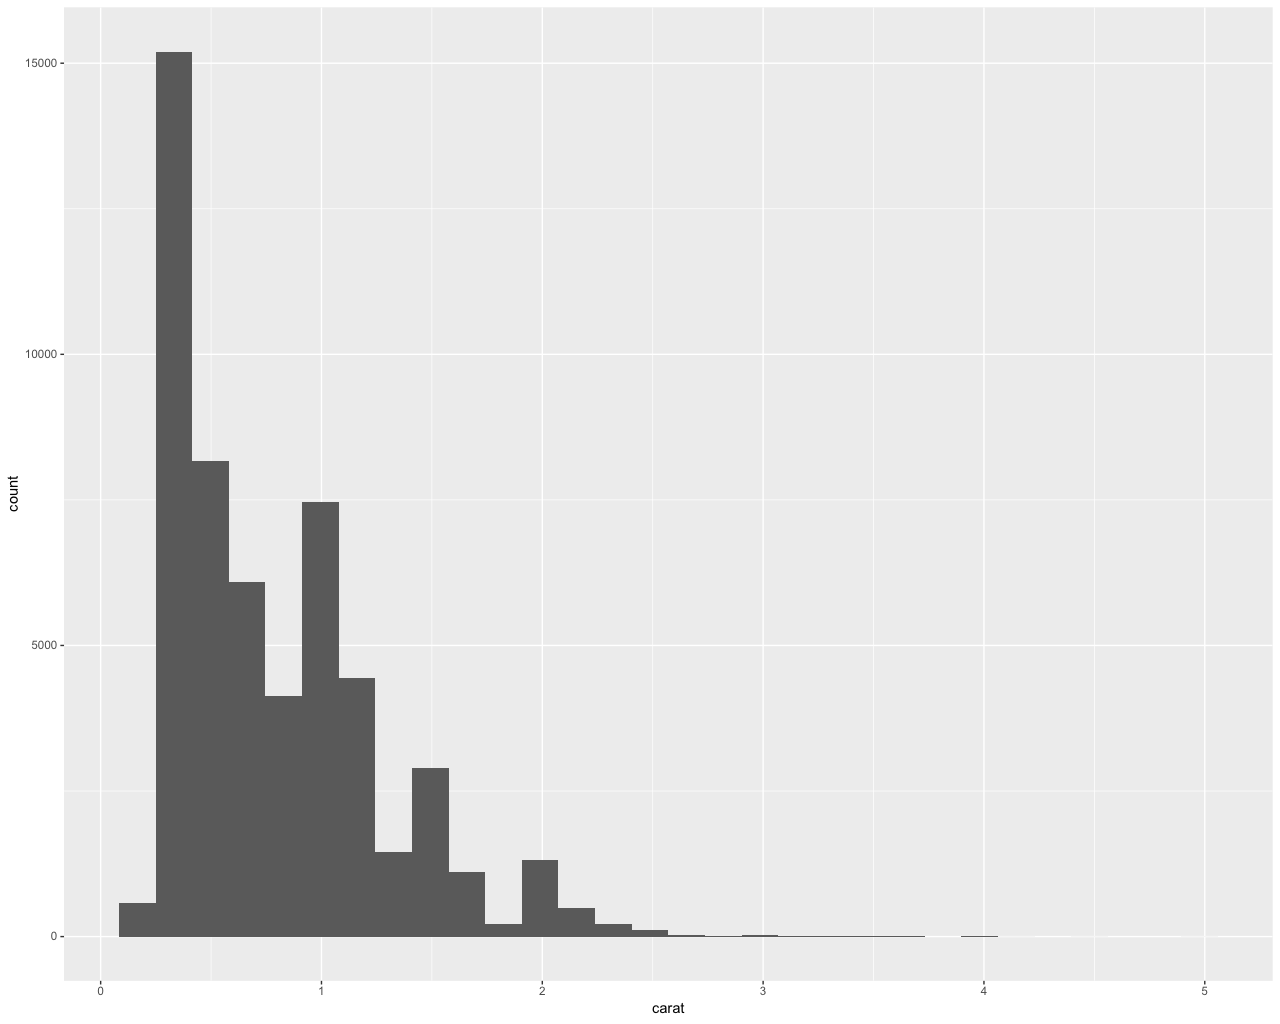
\includegraphics[width=\textwidth,height=0.75\textheight]{pic0030}\end{figure}
\end{frame}

\begin{frame}
\frametitle{Хистограма при 100 групи}
\begin{figure}[]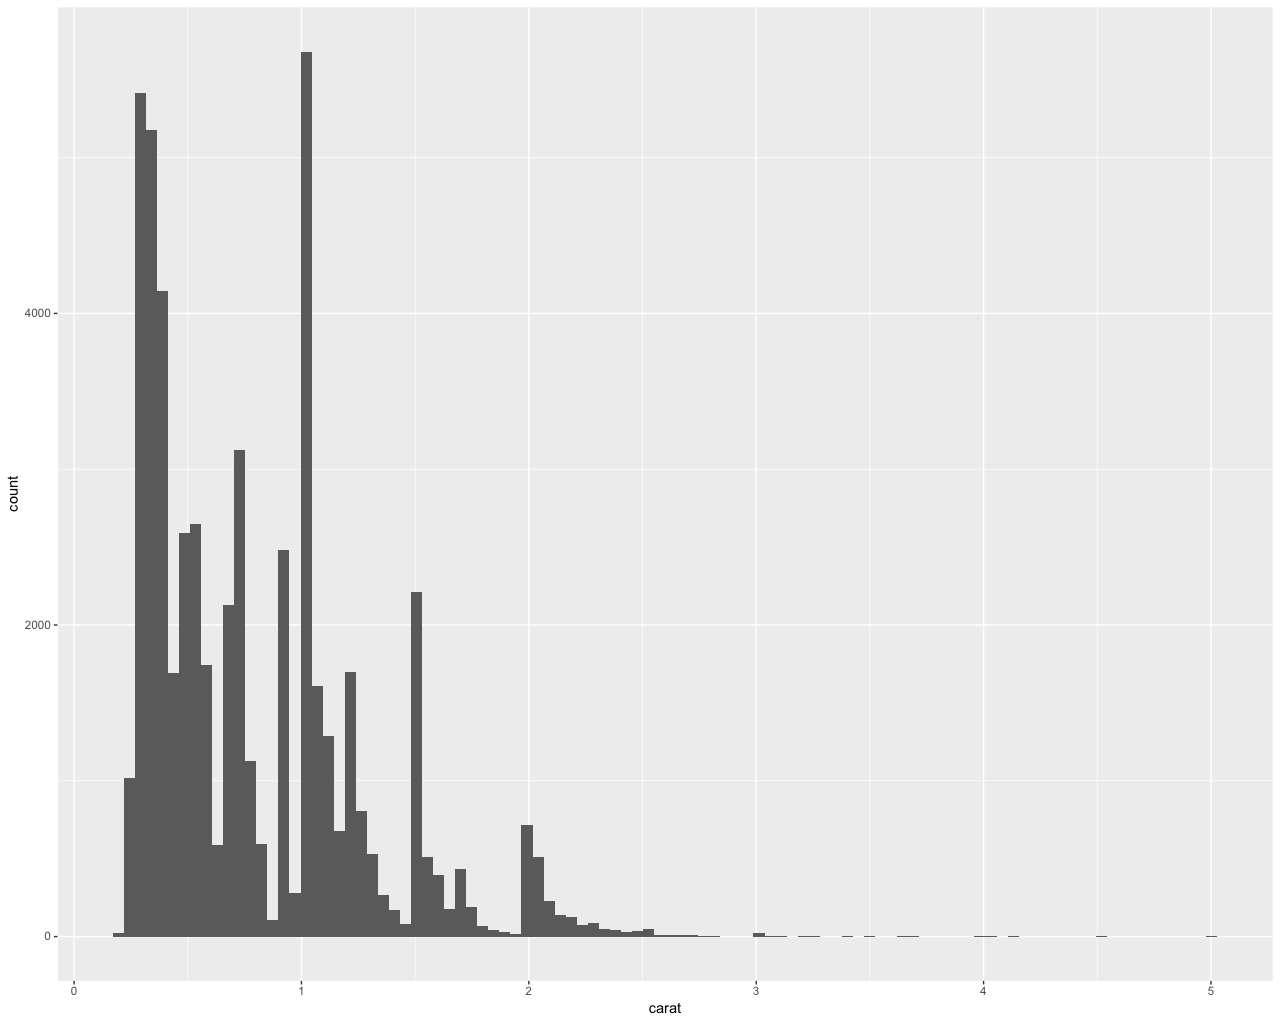
\includegraphics[width=\textwidth,height=0.75\textheight]{pic0031}\end{figure}
\end{frame}

\begin{frame}
\frametitle{Плътностна функция}
\begin{figure}[]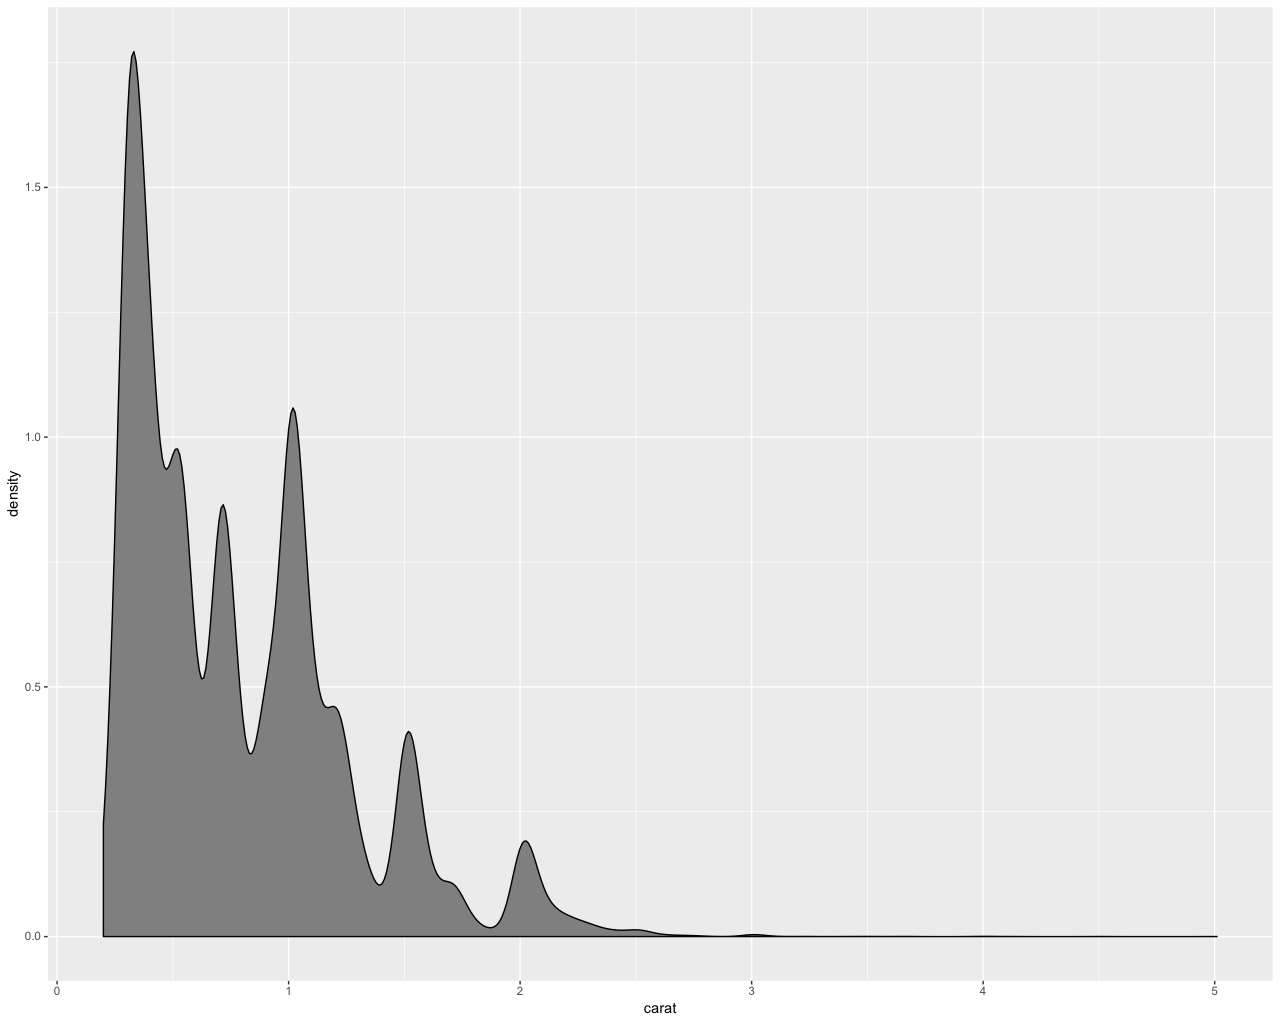
\includegraphics[width=\textwidth,height=0.75\textheight]{pic0032}\end{figure}
\end{frame}

\subsection{Диаграми на разсейване}

\begin{frame}
\frametitle{Визуализация при две променливи}
\begin{block}{Диаграма на разсейване с ggplot2}
library( ggplot2 )

ggplot(diamonds, aes(x=carat, y=price)) + geom\_point()
\end{block}
\end{frame}

\begin{frame}
\frametitle{Отношение на цена към тегло}
\begin{figure}[]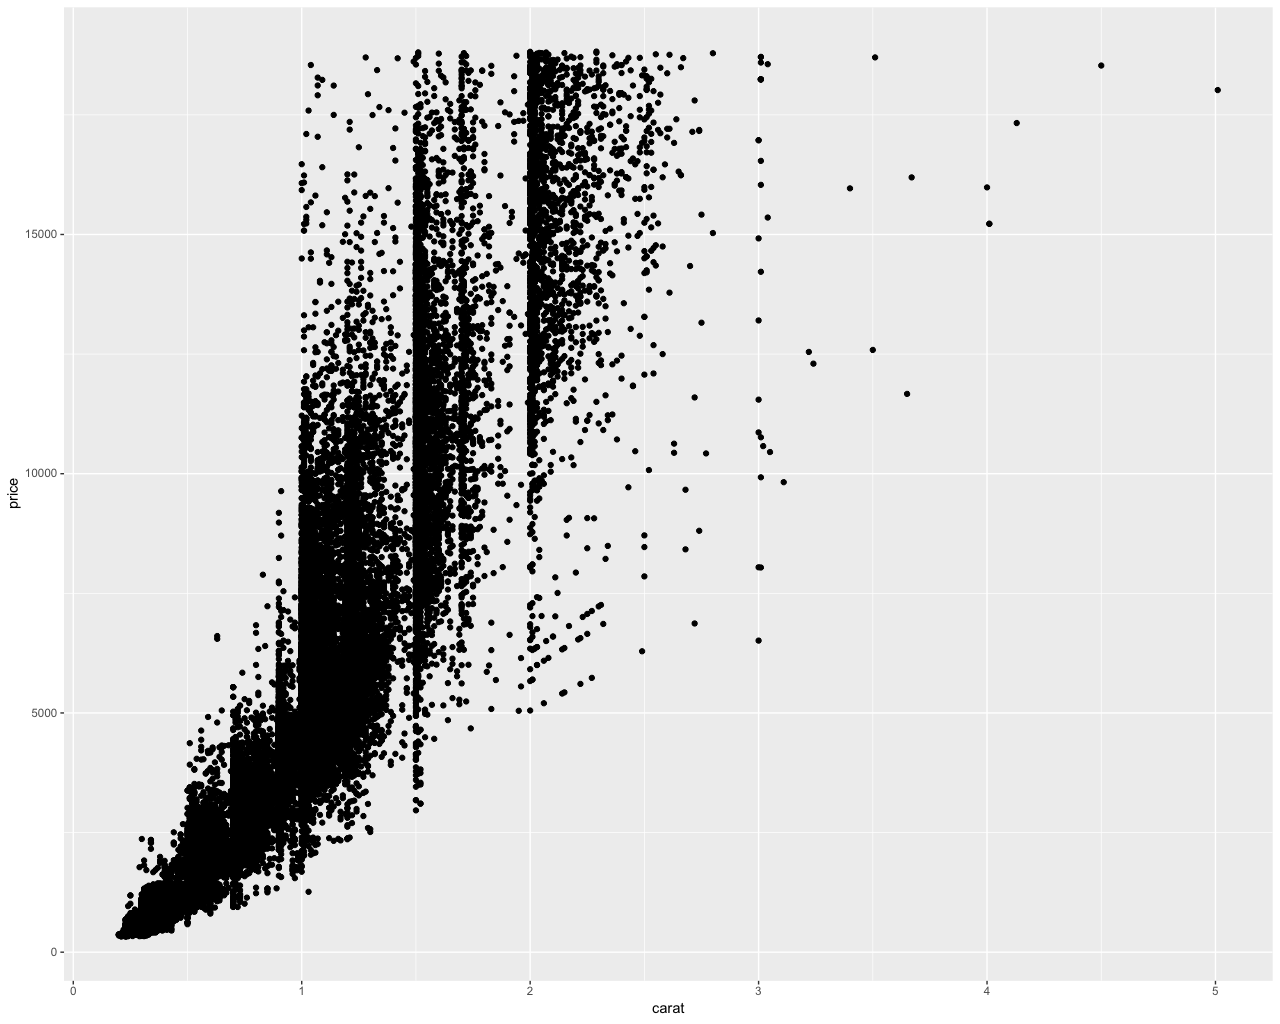
\includegraphics[width=\textwidth,height=0.75\textheight]{pic0033}\end{figure}
\end{frame}

\begin{frame}
\frametitle{Обработка по групи}
\begin{block}{Диаграма на разпръскване групирани по признак}
c2p <- ggplot(diamonds, aes(x=carat, y=price))

c2p + geom\_point(aes(color=color)) + facet\_wrap(\textasciitilde color)

c2p + geom\_point(aes(color=color)) + facet\_grid(clarity\textasciitilde cut)
\end{block}
\end{frame}

\begin{frame}
\frametitle{Диаграма на разпръскване по групи за цвят на диамантите}
\begin{figure}[]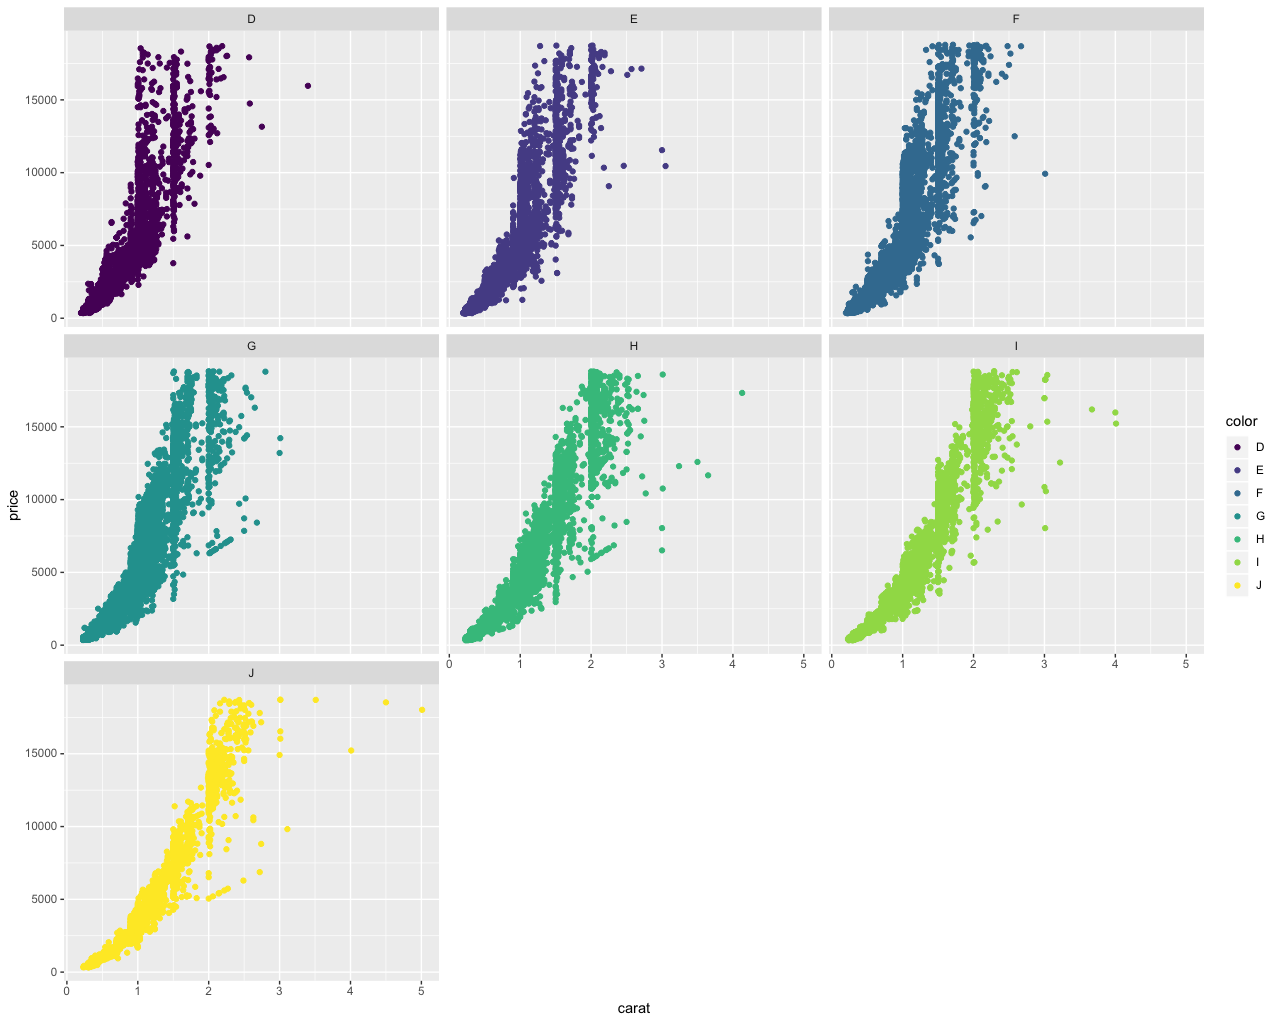
\includegraphics[width=\textwidth,height=0.75\textheight]{pic0034}\end{figure}
\end{frame}

\begin{frame}
\frametitle{Визуализация с групиране по два признака}
\begin{figure}[]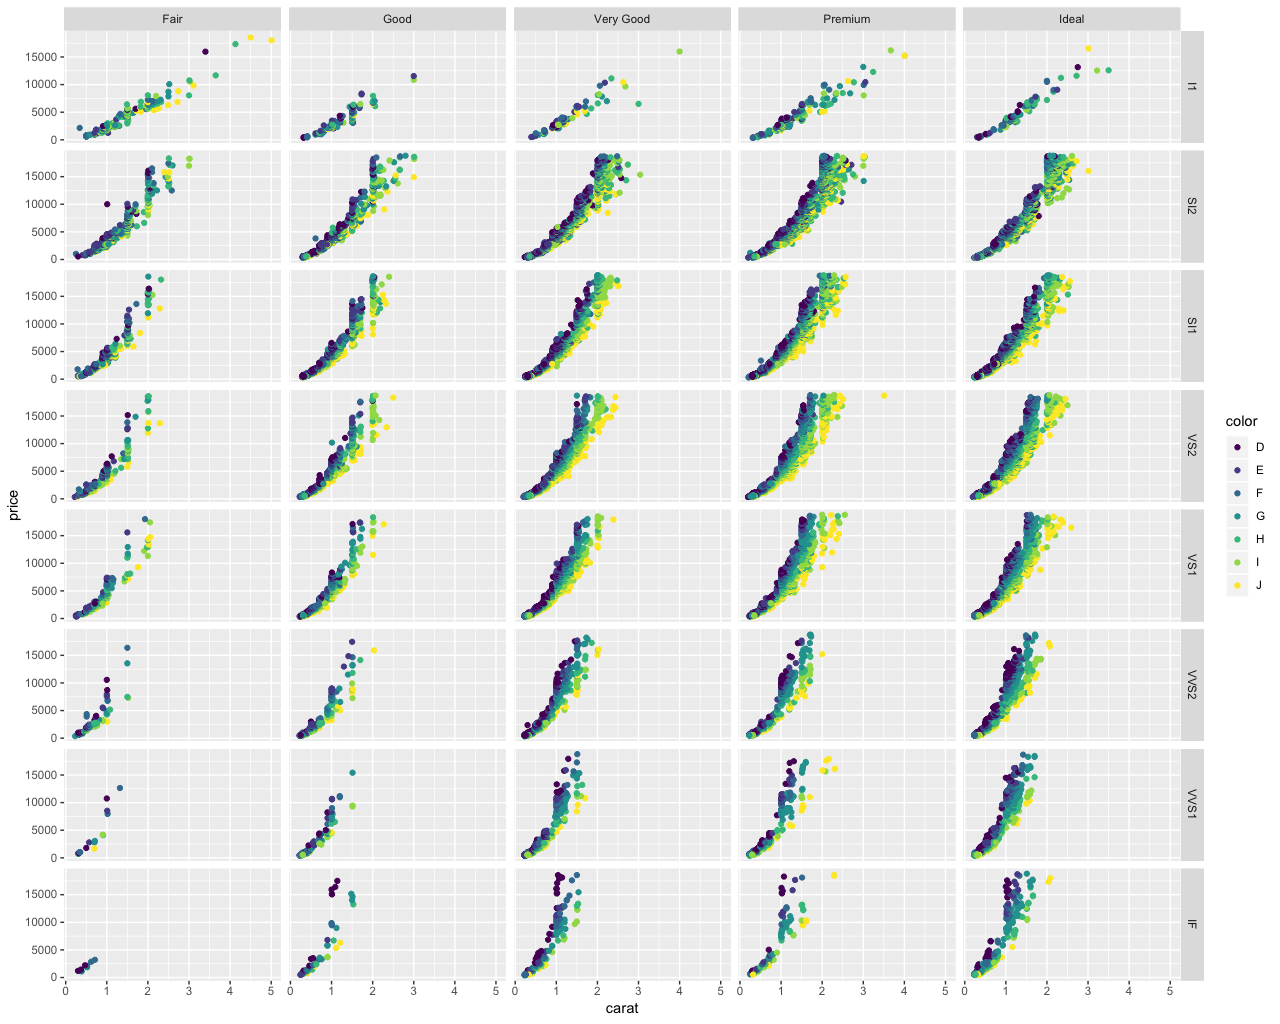
\includegraphics[width=\textwidth,height=0.75\textheight]{pic0035}\end{figure}
\end{frame}

\begin{frame}
\frametitle{Визуализация на хистограми с групиране}
\begin{figure}[]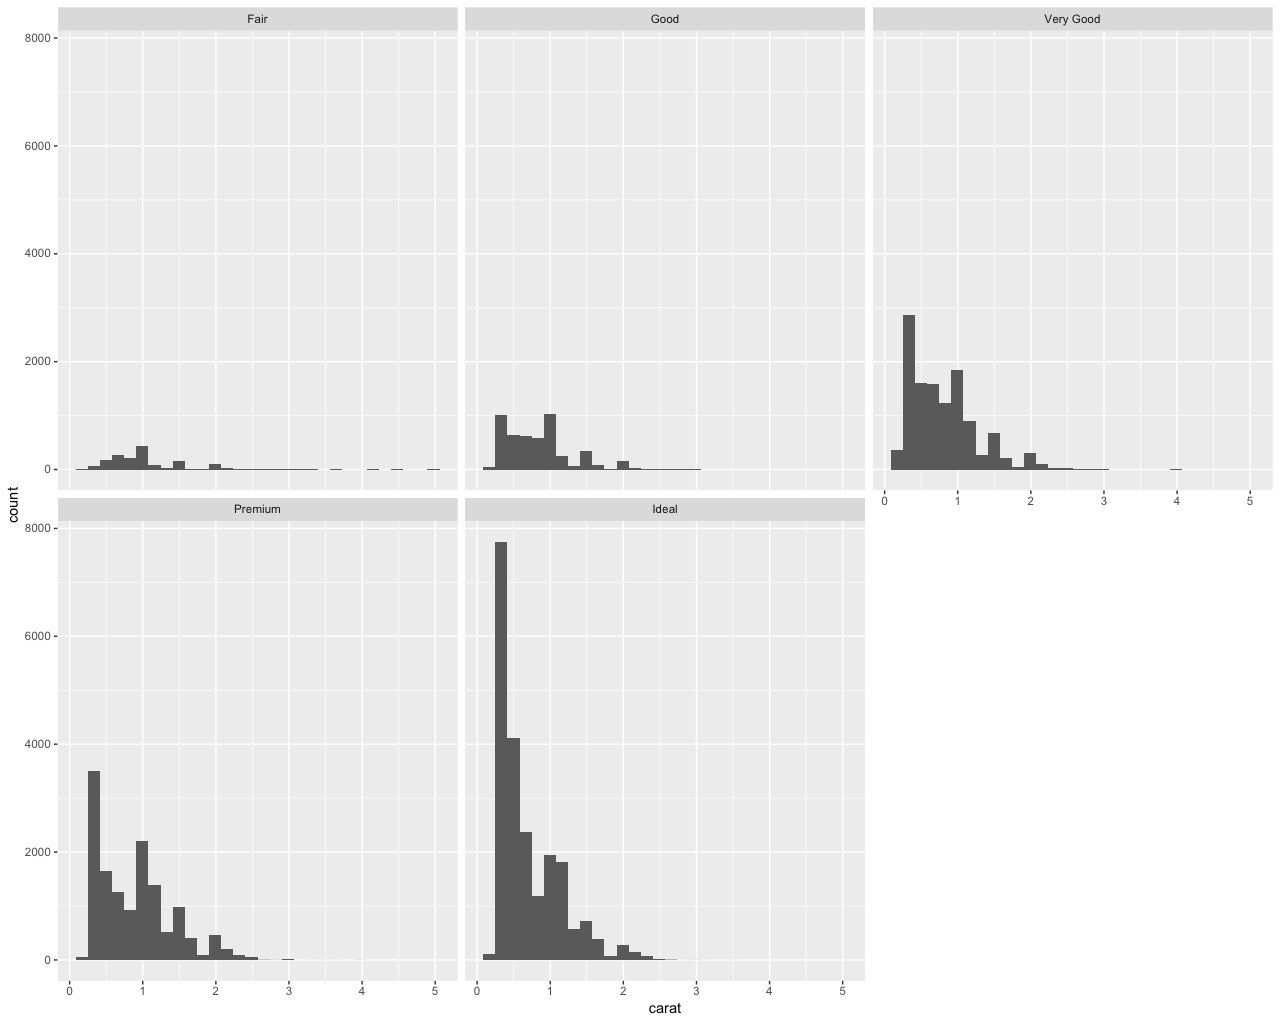
\includegraphics[width=\textwidth,height=0.75\textheight]{pic0036}\end{figure}
\end{frame}

\subsection{Графики тип кутия и цигулка}

\begin{frame}
\frametitle{Изобразяване на квартили}
\begin{block}{Визуализация тип кутия}
ggplot(diamonds, aes(y=depth)) + geom\_boxplot()

ggplot(diamonds, aes(y=depth, x=cut)) + geom\_boxplot()

ggplot(diamonds, aes(y=depth, x=cut)) + geom\_boxplot() + geom\_violin()

ggplot(diamonds, aes(y=depth, x=cut))+ geom\_point() + geom\_violin()
\end{block}
\end{frame}

\begin{frame}
\frametitle{Визуализация на характеристиката за дълбочина на диамантите}
\begin{figure}[]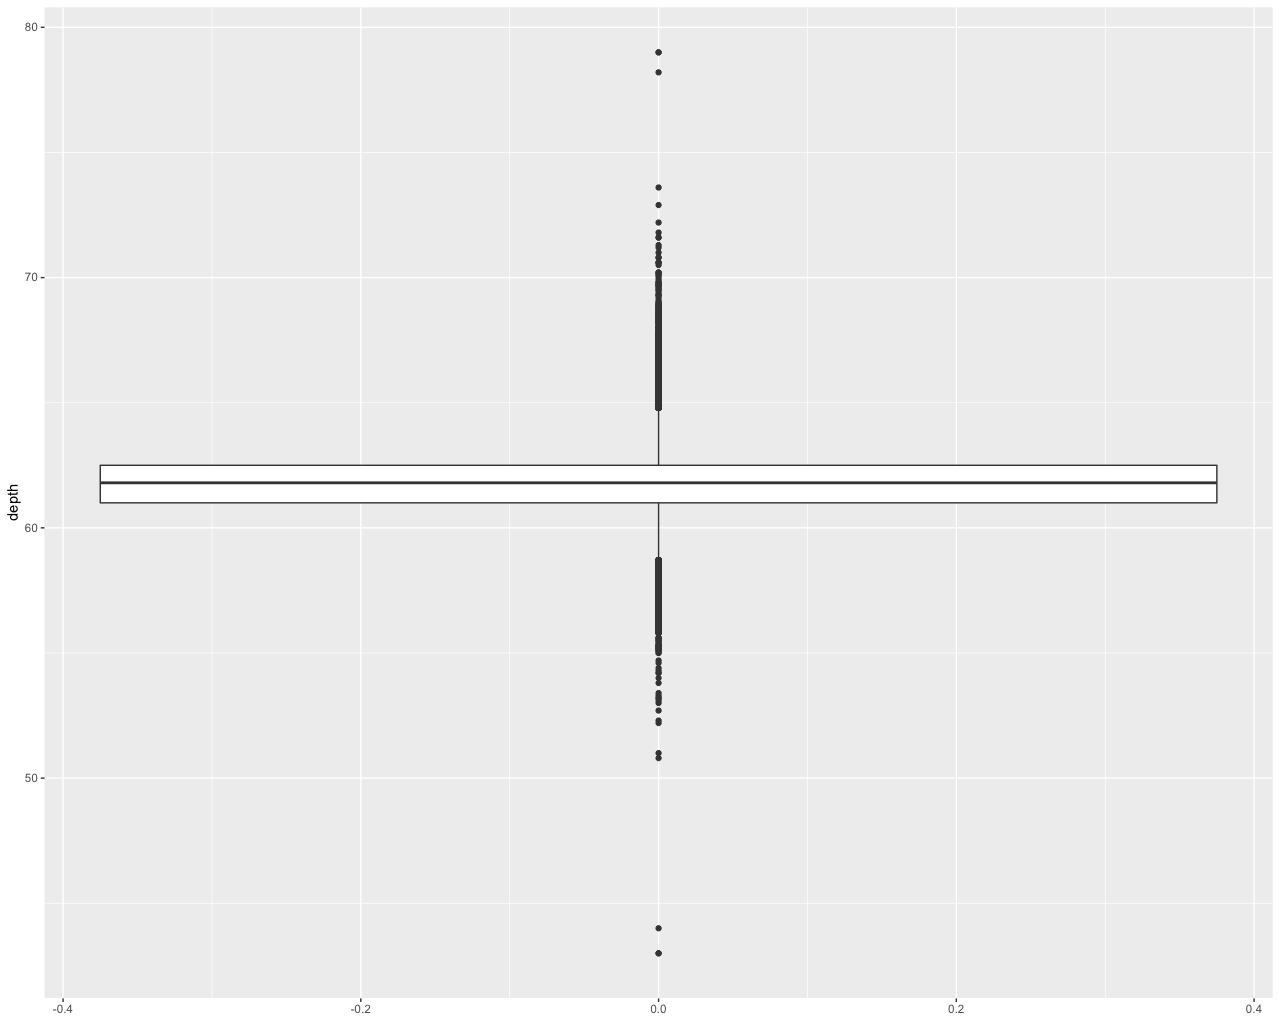
\includegraphics[width=\textwidth,height=0.75\textheight]{pic0037}\end{figure}
\end{frame}

\begin{frame}
\frametitle{Дълбочина на диамантите в групи според сряза}
\begin{figure}[]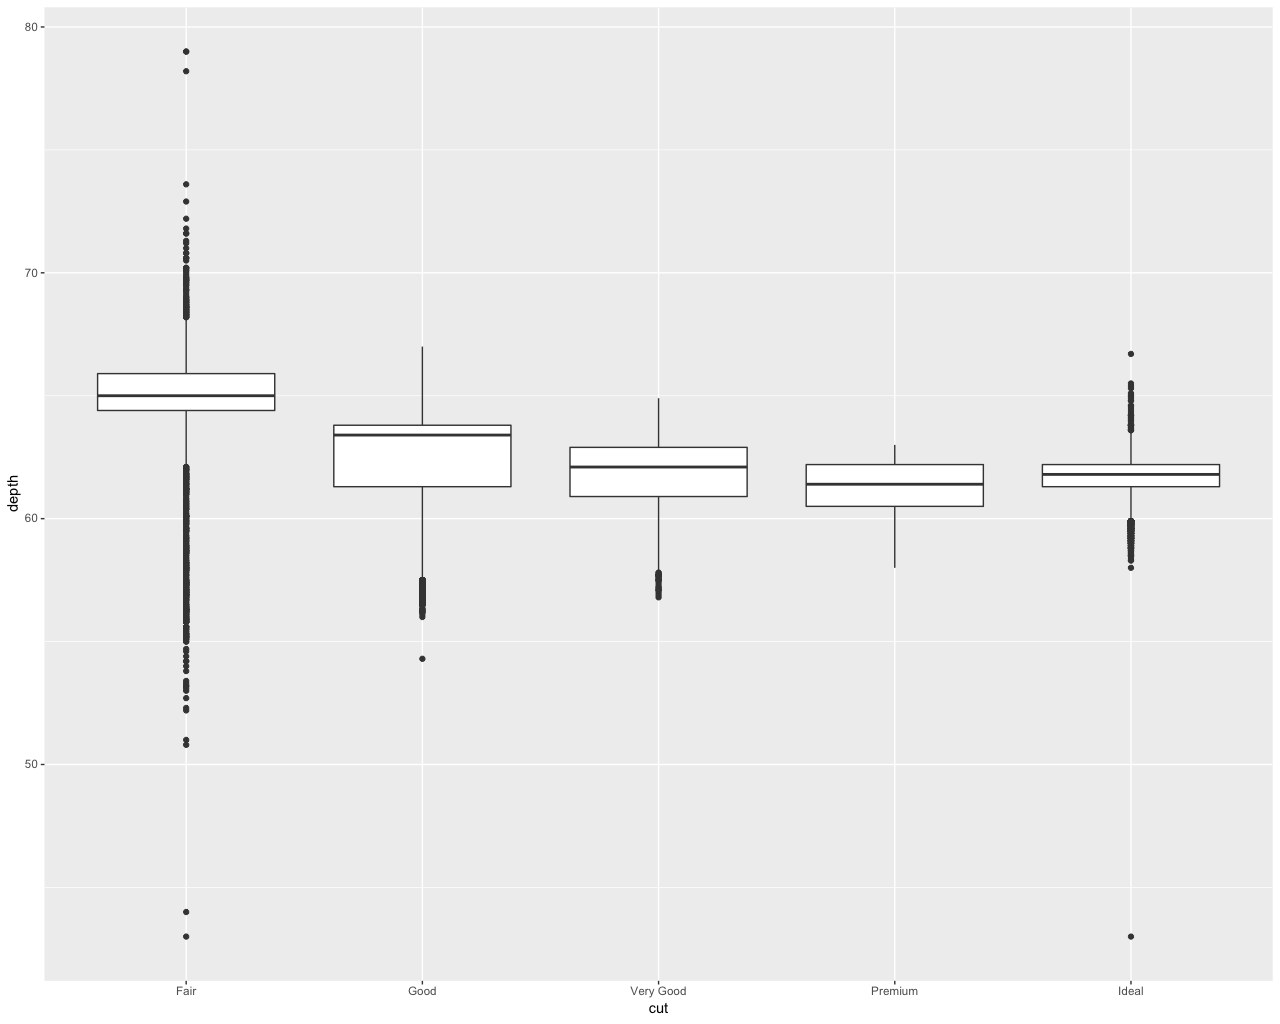
\includegraphics[width=\textwidth,height=0.75\textheight]{pic0038}\end{figure}
\end{frame}

\begin{frame}
\frametitle{Графика тип цигулки}
\begin{figure}[]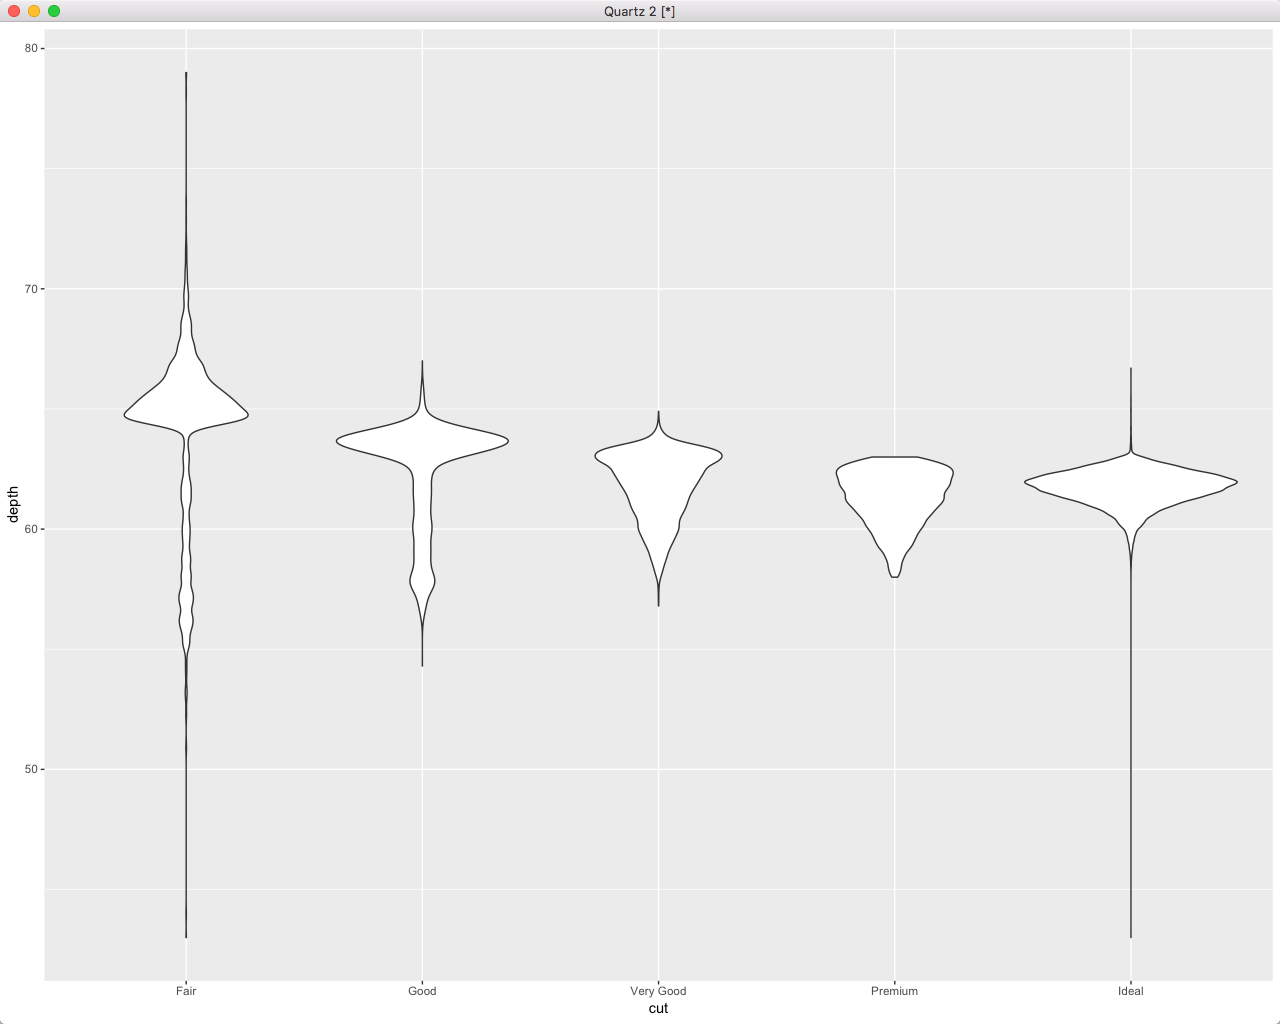
\includegraphics[width=\textwidth,height=0.75\textheight]{pic0039}\end{figure}
\end{frame}

\begin{frame}
\frametitle{Добавяне на декорация с точки}
\begin{figure}[]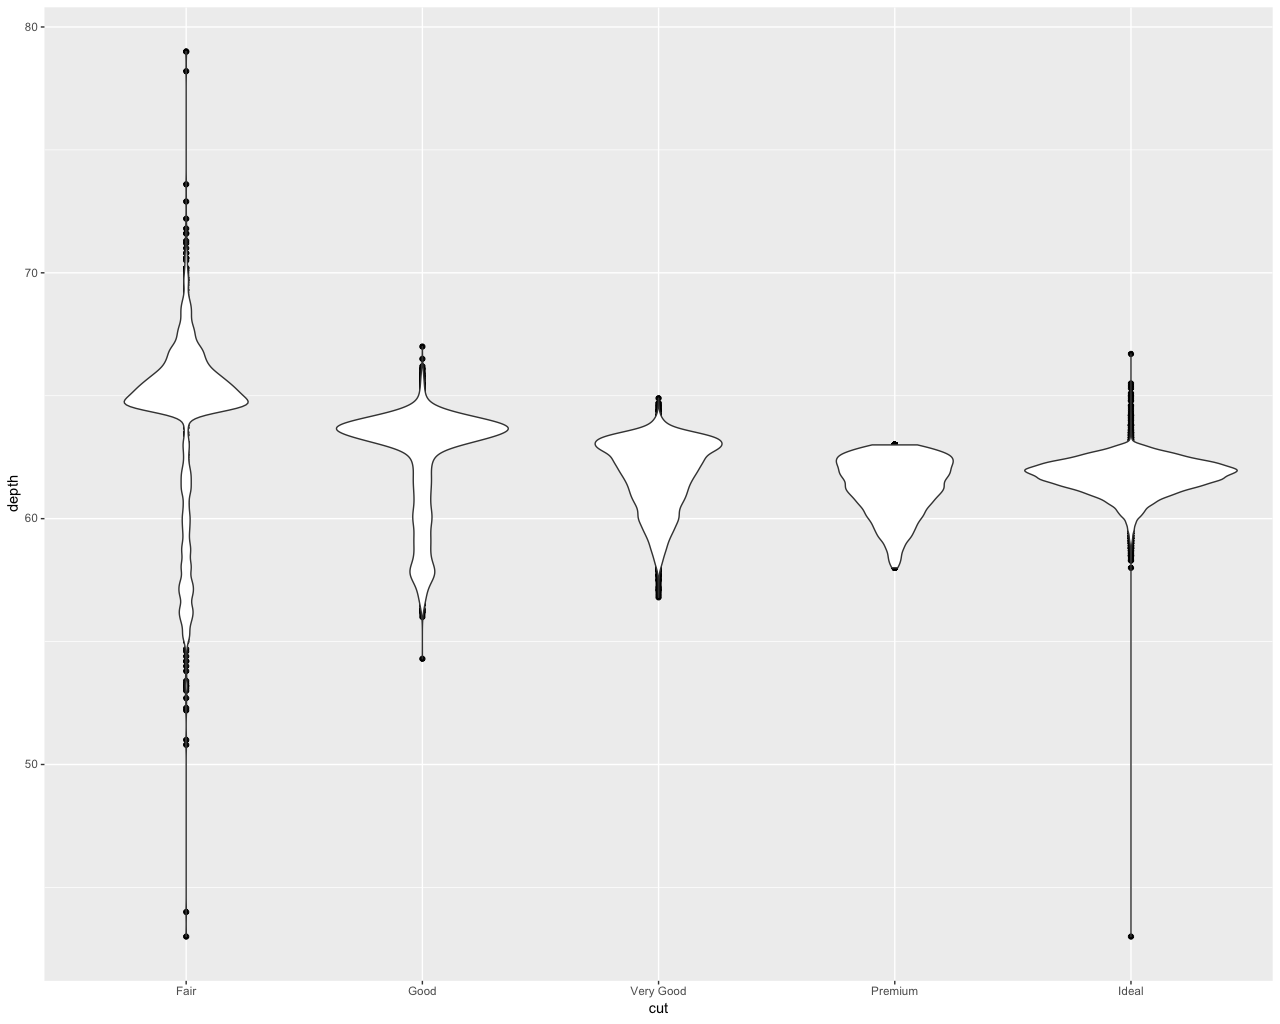
\includegraphics[width=\textwidth,height=0.75\textheight]{pic0040}\end{figure}
\end{frame}

\subsection{Линейни графики}

\begin{frame}
\frametitle{}
\begin{block}{Линейни графики}
library( lubridate )

ggplot(economics, aes(x=date, y=pop)) + geom\_line()

economics\$year <- year( economics\$date )

economics\$month <- month(economics\$date, label=TRUE)

library( scales )

ggplot(economics, aes(x=month, y=pop)) + geom\_line(aes(color=factor(year), group=year)) + scale\_color\_discrete(name=$"$Year$"$) + scale\_y\_continuous(labels=comma)+ labs(title=$"$Population Growth$"$, x=$"$Month$"$, y=$"$Population$"$)
\end{block}
\end{frame}

\begin{frame}
\frametitle{Нарастване на популацията във времето}
\begin{figure}[]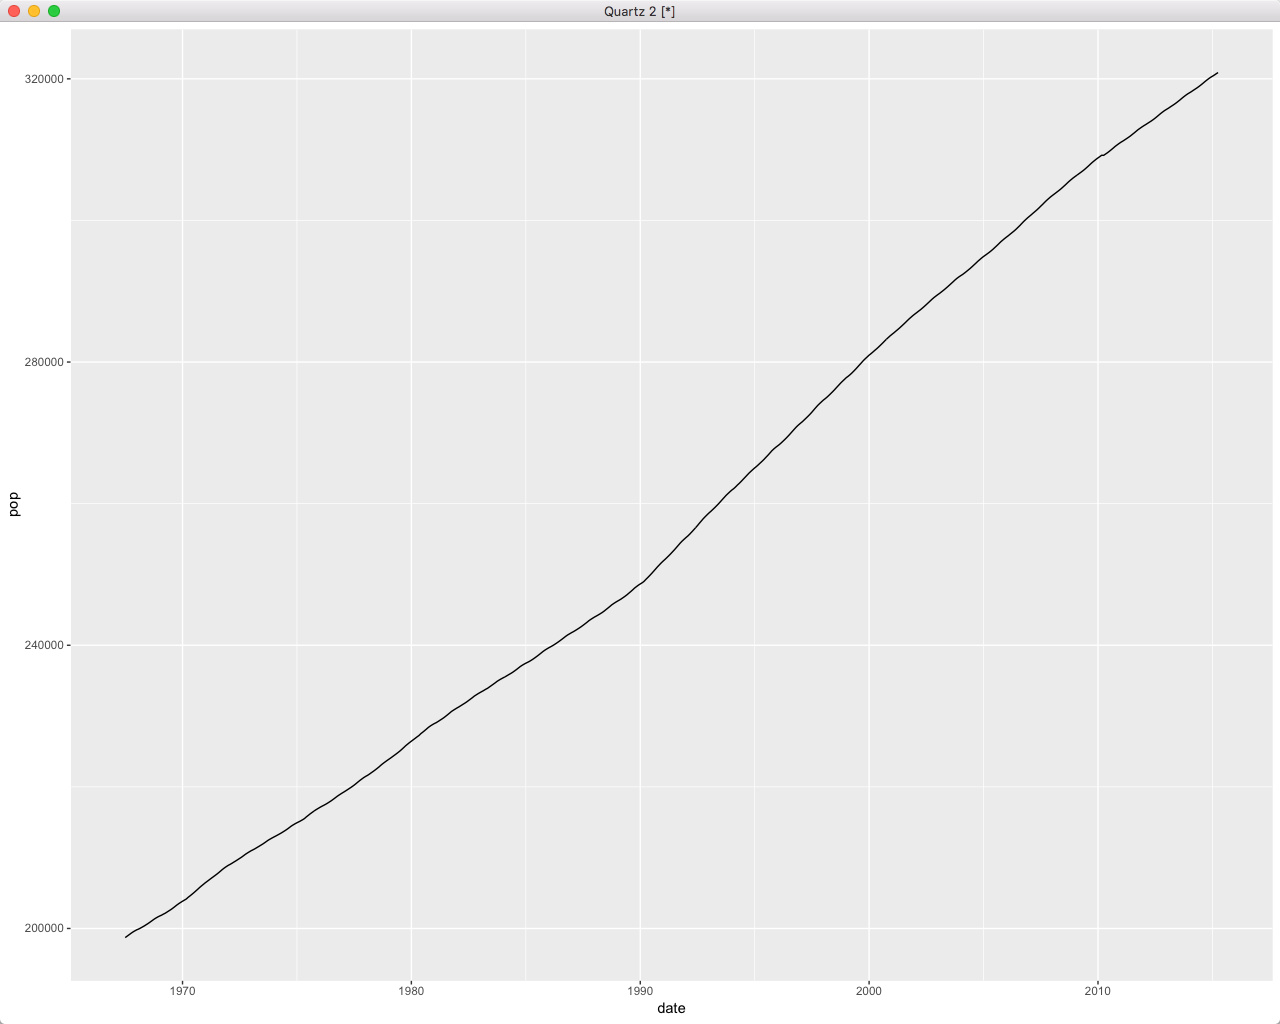
\includegraphics[width=\textwidth,height=0.75\textheight]{pic0041}\end{figure}
\end{frame}

\begin{frame}
\frametitle{Визуализиране на приръста по години}
\begin{figure}[]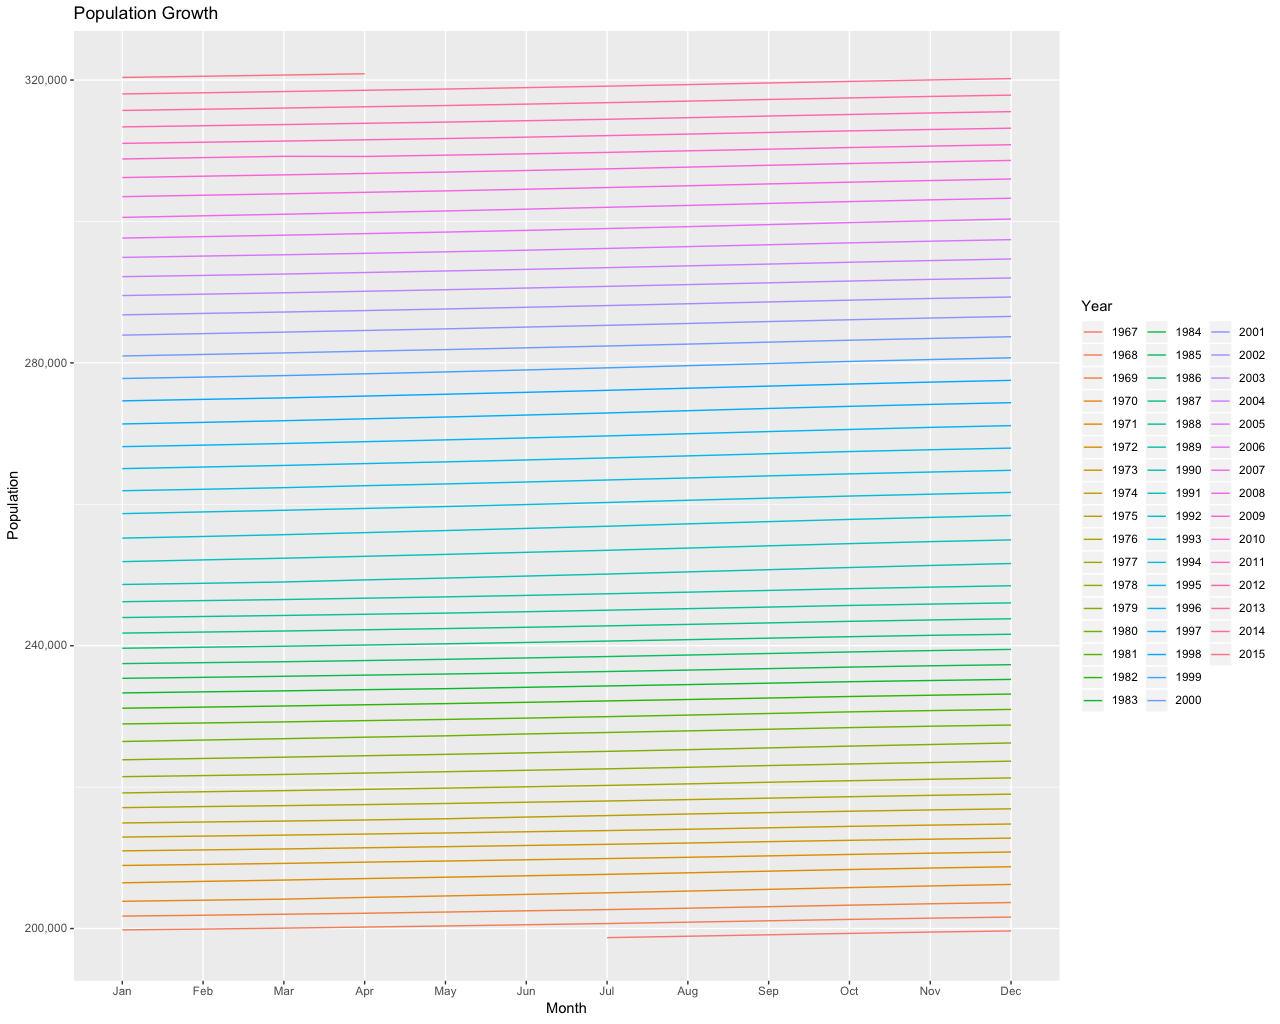
\includegraphics[width=\textwidth,height=0.75\textheight]{pic0042}\end{figure}
\end{frame}

\subsection{Тематично оформление}

\begin{frame}
\frametitle{Визуализация за подходяща медия}
\begin{block}{Избор на теми за визуално представяне}
library( ggthemes )

ggplot(diamonds, aes(x=carat, y=price)) + geom\_point(aes(color=color)) + theme\_wsj()

ggplot(diamonds, aes(x=carat, y=price)) + geom\_point(aes(color=color)) + theme\_tufte()

ggplot(diamonds, aes(x=carat, y=price)) + geom\_point(aes(color=color)) + theme\_excel()

ggplot(diamonds, aes(x=carat, y=price)) + geom\_point(aes(color=color)) +  theme\_economist() + scale\_colour\_economist()
\end{block}
\end{frame}

\begin{frame}
\frametitle{Тема Wall Street Journal}
\begin{figure}[]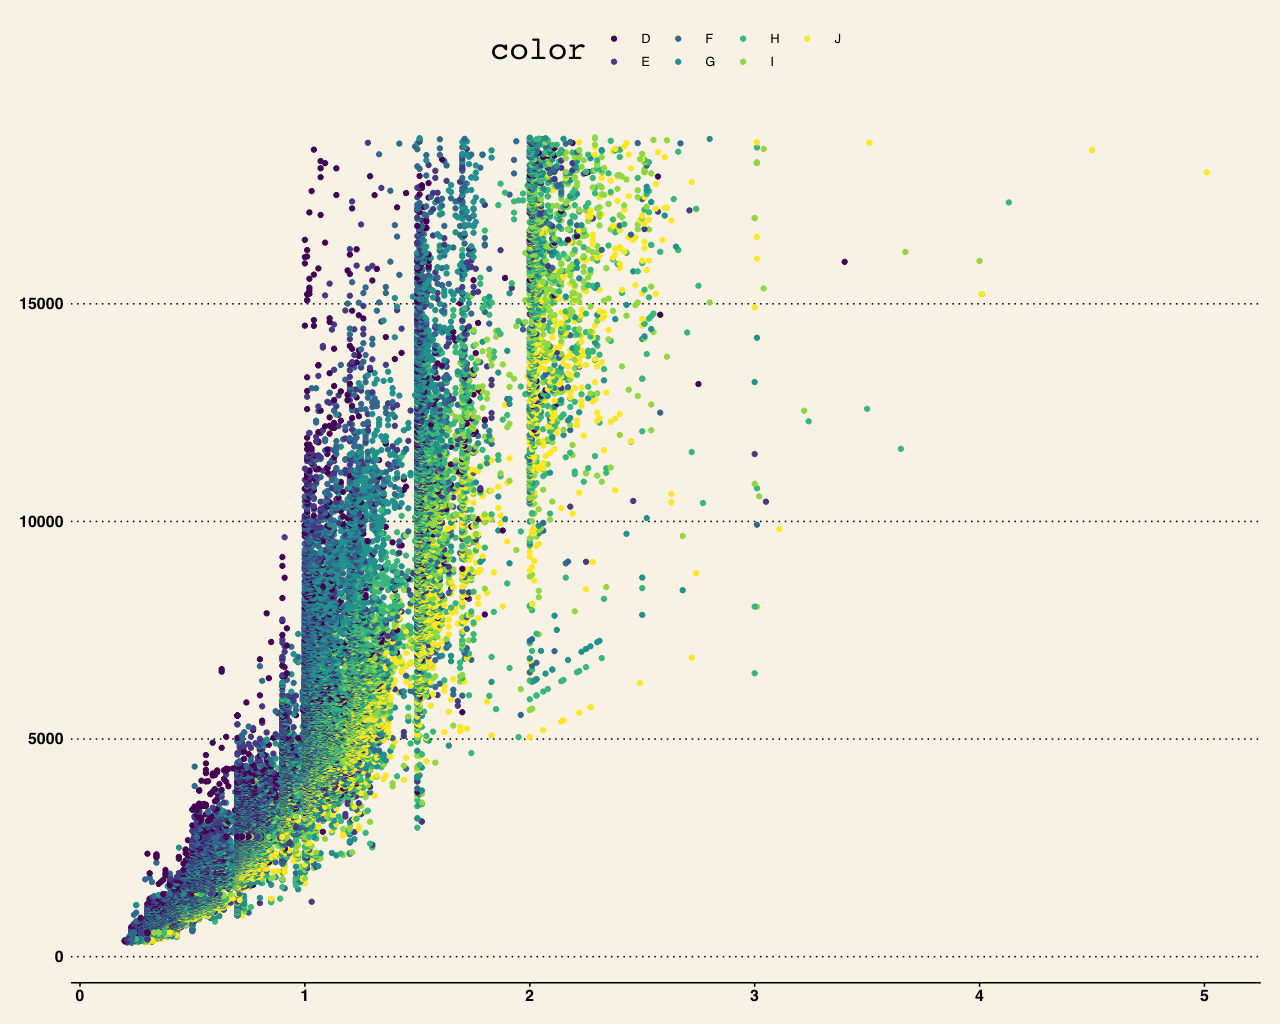
\includegraphics[width=\textwidth,height=0.75\textheight]{pic0043}\end{figure}
\end{frame}

\begin{frame}
\frametitle{Тема Edward Tufte}
\begin{figure}[]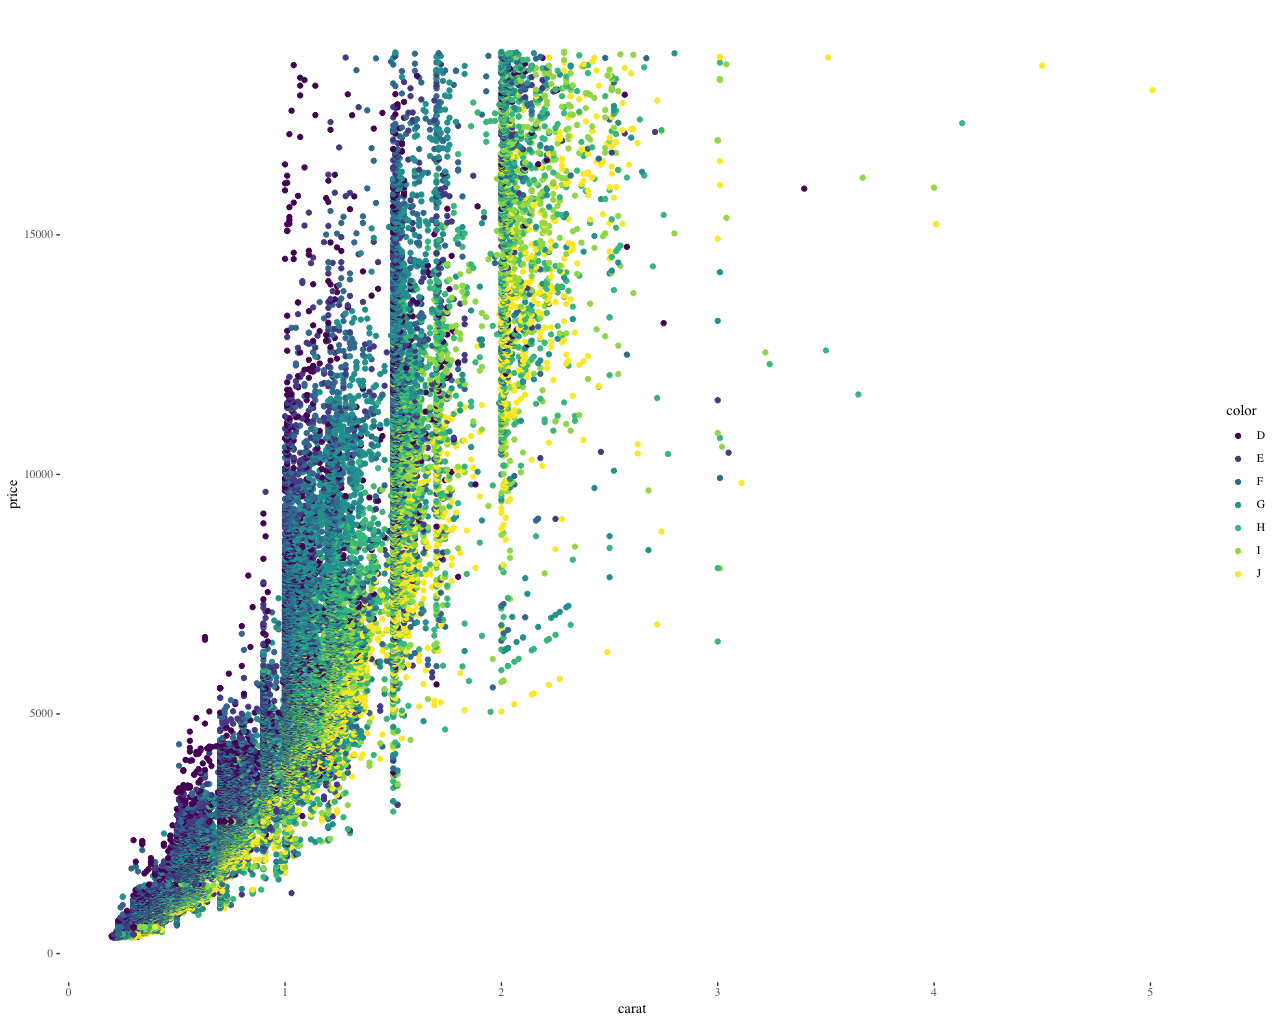
\includegraphics[width=\textwidth,height=0.75\textheight]{pic0044}\end{figure}
\end{frame}

\begin{frame}
\frametitle{Тема в стил Microsoft Excel}
\begin{figure}[]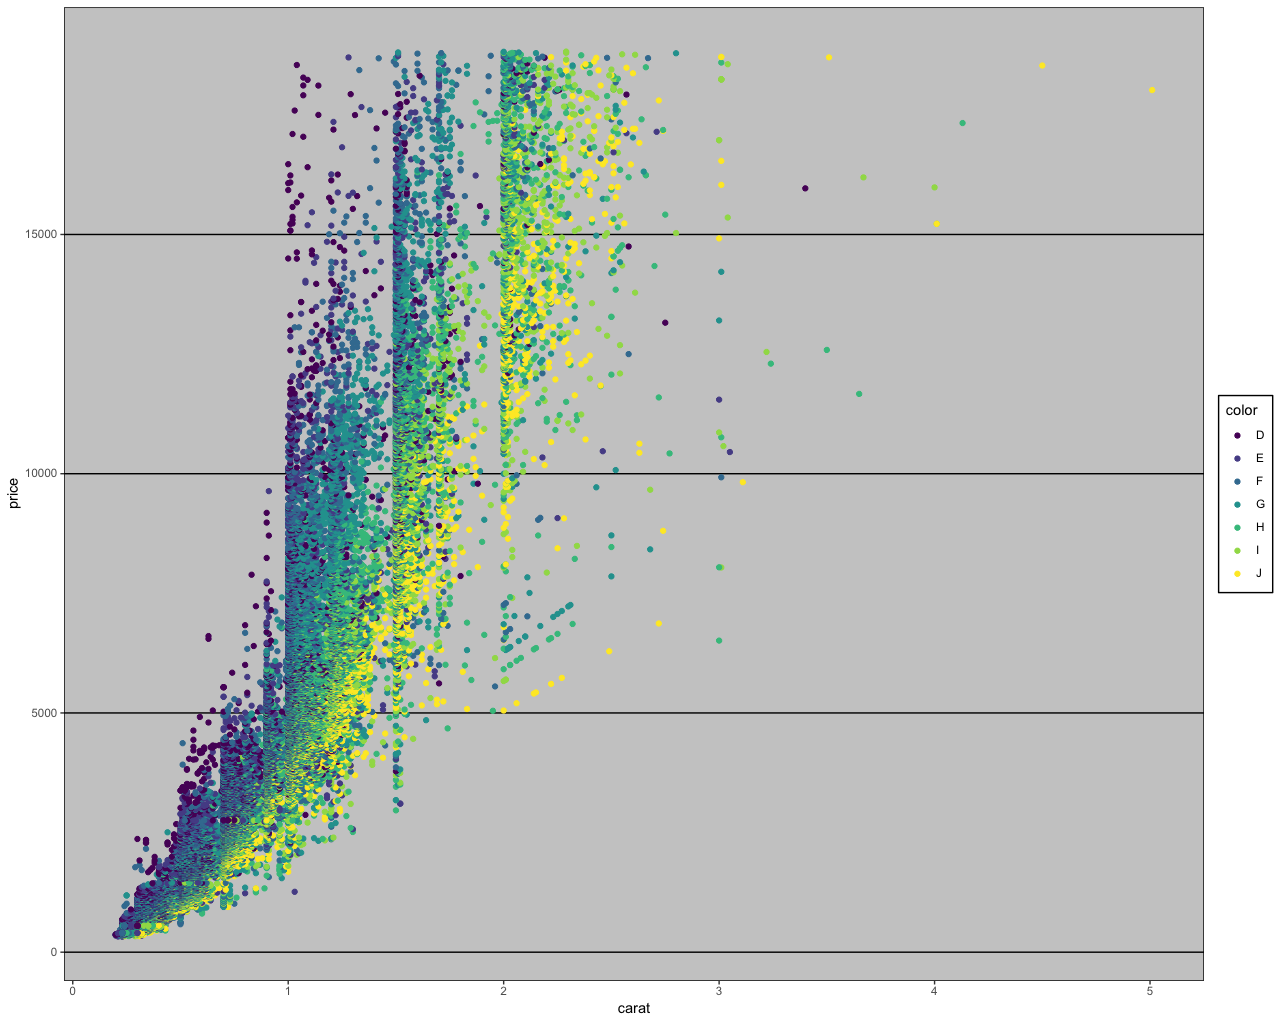
\includegraphics[width=\textwidth,height=0.75\textheight]{pic0045}\end{figure}
\end{frame}

\begin{frame}
\frametitle{Тема Economist}
\begin{figure}[]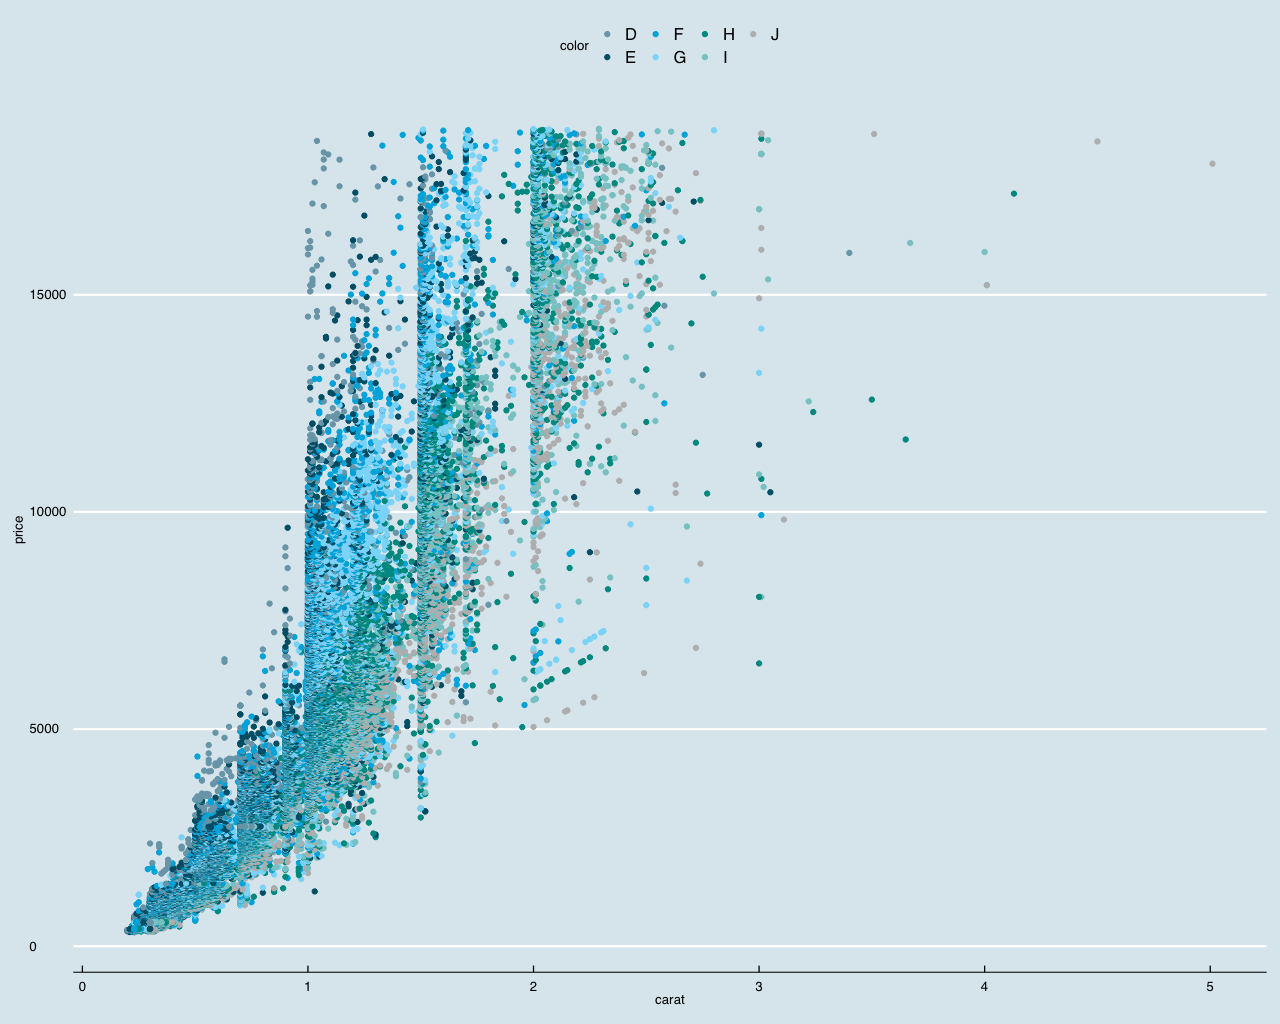
\includegraphics[width=\textwidth,height=0.75\textheight]{pic0046}\end{figure}
\end{frame}

\section{Изследване на случайни величини}

\begin{frame}
\center \huge{Изследване на случайни величини}
\end{frame}

\subsection{Зарове за игра}

\begin{frame}
\frametitle{Случайни стойности от зарове}
\begin{block}{При един зар}
library( ggplot2 )

library( Rdice )

x <- dice.roll(faces=6, dice=1, rolls=100000)

ggplot(data=x\$results) + geom\_histogram(aes(x=values)) + ggtitle($"$Single die rolled 100K times.$"$) + xlab($"$Die Side$"$) + ylab($"$Outcomes$"$) + scale\_x\_continuous(breaks=round(seq(min(x\$results\$values), max(x\$results\$values),by=0.5)))
\end{block}
\end{frame}

\begin{frame}
\frametitle{Хистограма на хвърлянията за един зар}
\begin{figure}[]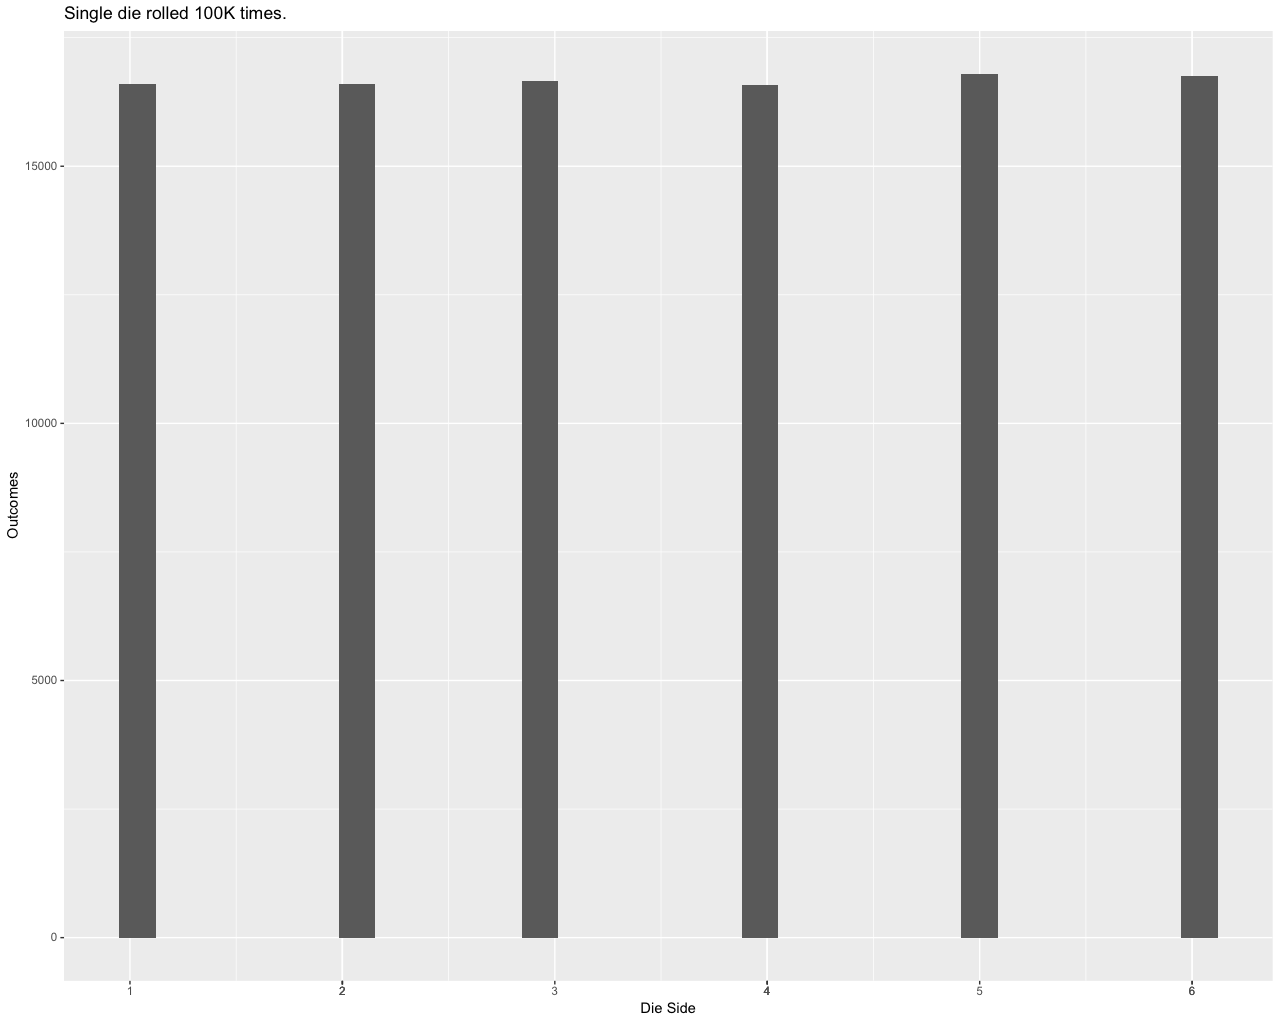
\includegraphics[width=\textwidth,height=0.75\textheight]{pic0047}\end{figure}
\end{frame}

\begin{frame}
\frametitle{Случайни стойности от зарове}
\begin{block}{При два зара}
x <- dice.roll(faces=6, dice=2, rolls=100000)

ggplot(data=x\$results) + geom\_histogram(aes(x=(die\_1+die\_2))) + ggtitle($"$Two dice rolled 100K times.$"$) + xlab($"$Dice Sides$"$) + ylab($"$Outcomes$"$) + scale\_x\_continuous(breaks=round(seq(min((x\$results\$die\_1 + x\$results\$die\_2)), max((x\$results\$die\_1+x\$results\$die\_2)),by=0.5)))
\end{block}
\end{frame}

\begin{frame}
\frametitle{Хистограма на хвърлянията за два зара}
\begin{figure}[]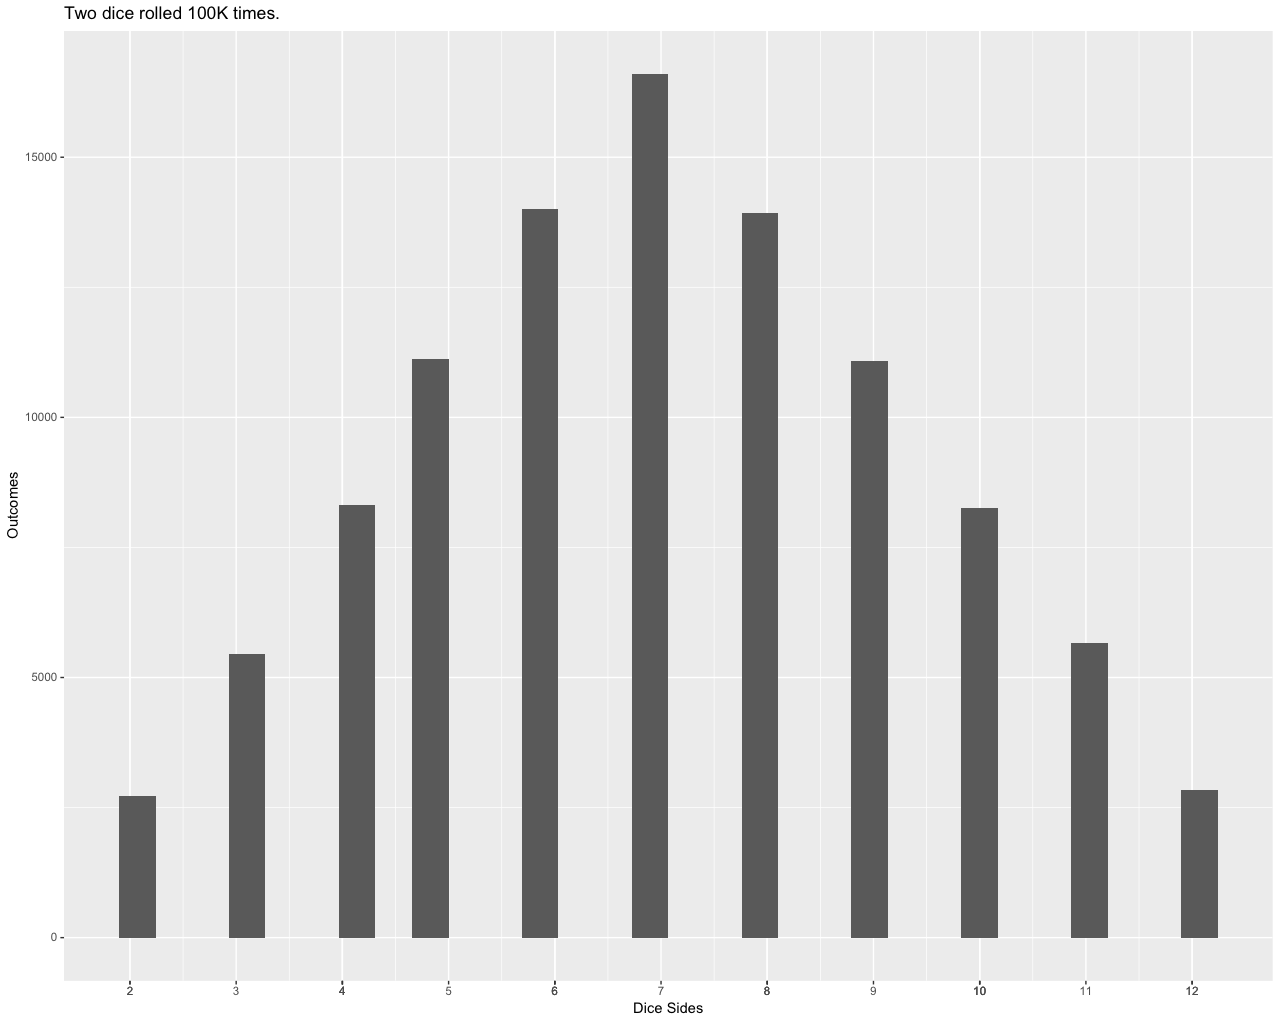
\includegraphics[width=\textwidth,height=0.75\textheight]{pic0048}\end{figure}
\end{frame}

\begin{frame}
\frametitle{Случайни стойности от зарове}
\begin{block}{При шест зара}
x <- dice.roll(faces=6, dice=6, rolls=100000)

x\$results\$values = rowSums( x\$results[,1:6] )

ggplot(data=x\$results) + geom\_histogram(aes(x=values)) + ggtitle($"$Six dice rolled 100K times.$"$) + xlab($"$Dice Sides$"$) + ylab($"$Outcomes$"$) + scale\_x\_continuous(breaks=round(seq(min(x\$results\$values), max(x\$results\$values),by=0.5)))
\end{block}
\end{frame}

\begin{frame}
\frametitle{Хистограма на хвърлянията за шест зара}
\begin{figure}[]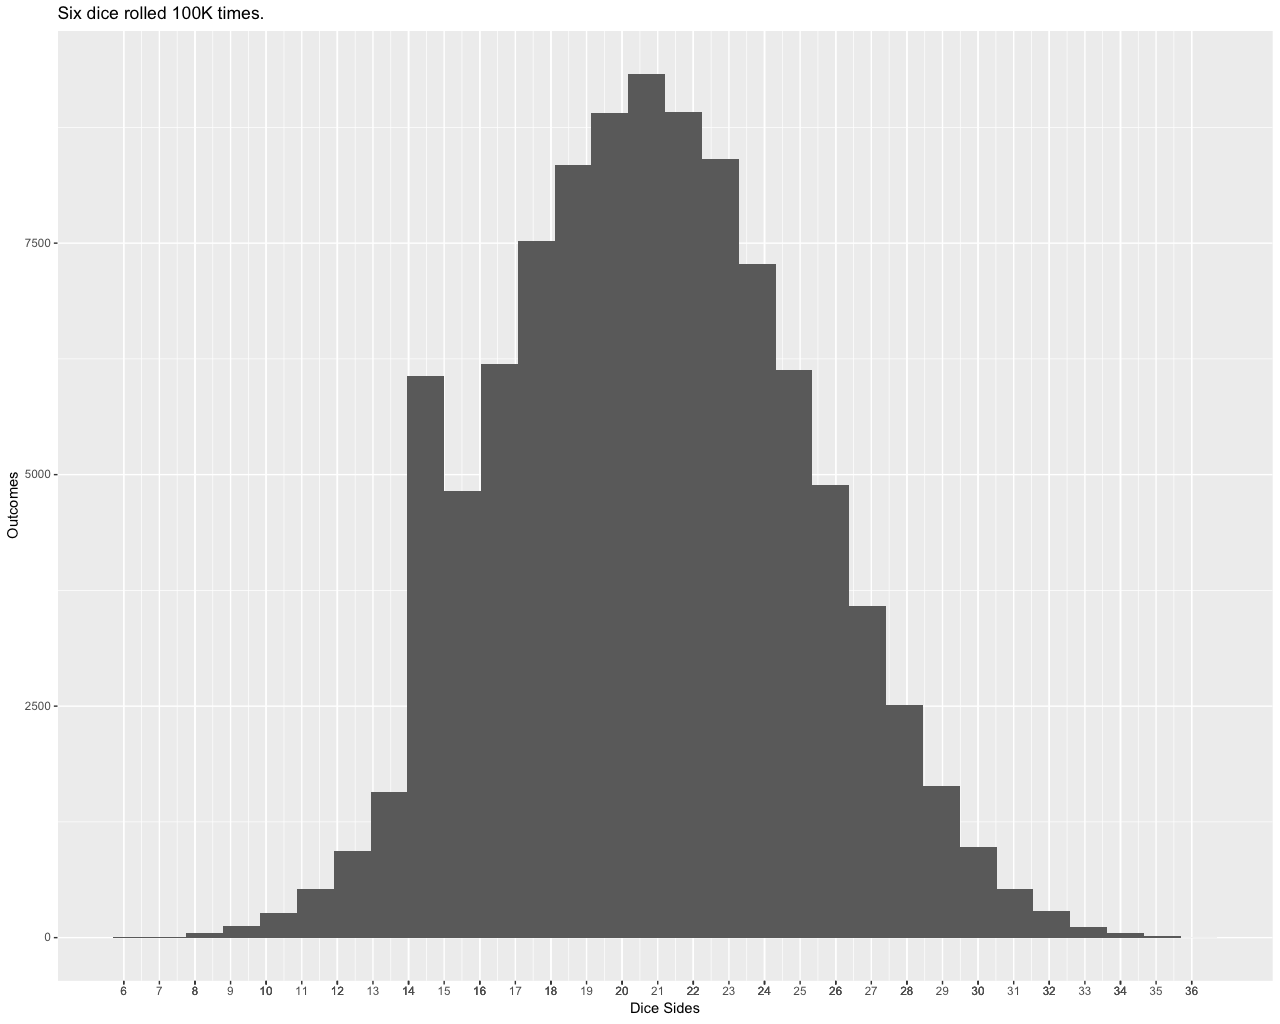
\includegraphics[width=\textwidth,height=0.75\textheight]{pic0049}\end{figure}
\end{frame}

\begin{frame}
\frametitle{Случайни стойности от зарове}
\begin{block}{При десет зара}
x <- dice.roll(faces=6, dice=10, rolls=100000)

x\$results\$values = rowSums( x\$results[,1:10] )

ggplot(data=x\$results) + geom\_density(aes(x=values)) + ggtitle($"$Ten dice rolled 100K times.$"$) + xlab($"$Dice Sides$"$) + ylab($"$Outcomes$"$) + scale\_x\_continuous(breaks=round(seq(min(x\$results\$values), max(x\$results\$values),by=0.5)))
\end{block}
\end{frame}

\begin{frame}
\frametitle{Плътностна диаграма на хвърлянията за десет зара}
\begin{figure}[]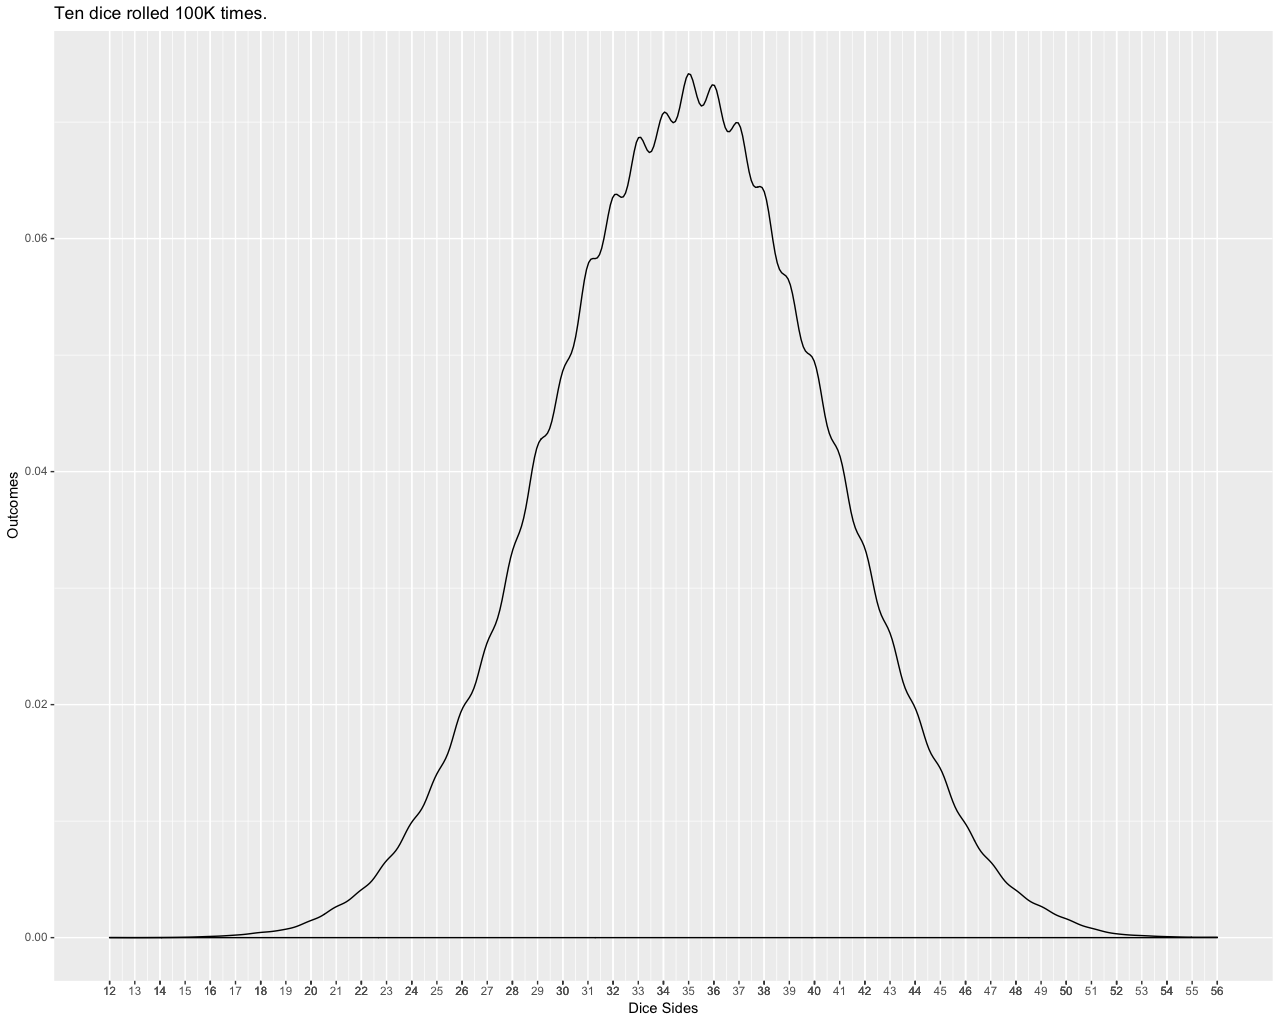
\includegraphics[width=\textwidth,height=0.75\textheight]{pic0050}\end{figure}
\end{frame}

\section{Вероятностни разпределения}

\begin{frame}
\center \huge{Вероятностни разпределения}
\end{frame}

\subsection{Нормално разпределение}

\begin{frame}
\frametitle{Вероятностна функция на нормално разпределение}
\begin{equation}
pdf(x) = \frac{1}{{\sigma \sqrt {2\pi } }}e^{{{ - \left( {x - \mu } \right)^2 } \mathord{\left/ {\vphantom {{ - \left( {x - \mu } \right)^2 } {2\sigma ^2 }}} \right. \kern-\nulldelimiterspace} {2\sigma ^2 }}}
\end{equation}
\end{frame}

\begin{frame}
\frametitle{Генериране, плътност, кумулативна функция, квантили}
\begin{block}{Функции за работа с нормално разпределение}
values <- rnorm(n=30000, mean=0, sd=0.85)

density <- dnorm( values ) 

cumulative <- pnorm( values ) 

quantile <- qnorm( cumulative )
\end{block}
\end{frame}

\begin{frame}
\frametitle{Плътност, кумулативна функция, квантили}
\begin{block}{Визуализация на графики за нормално разпределение}
ggplot(data.frame(x=values, y=density)) + aes(x=x, y=y) + geom\_line() + labs(x=$"$Normally Distributed Random Values$"$, y=$"$Density$"$)

ggplot(data.frame(x=values, y=cumulative)) + aes(x=x, y=y) + geom\_line() + labs(x=$"$Normally Distributed Random Values$"$, y=$"$Cumulative Probability$"$)

ggplot(data.frame(x=values, y=quantile)) + aes(x=x, y=y) + geom\_line() + labs(x=$"$Normally Distributed Random Values$"$, y=$"$Quantile$"$)
\end{block}
\end{frame}

\begin{frame}
\frametitle{Плътностна функция на нормално разпределение}
\begin{figure}[]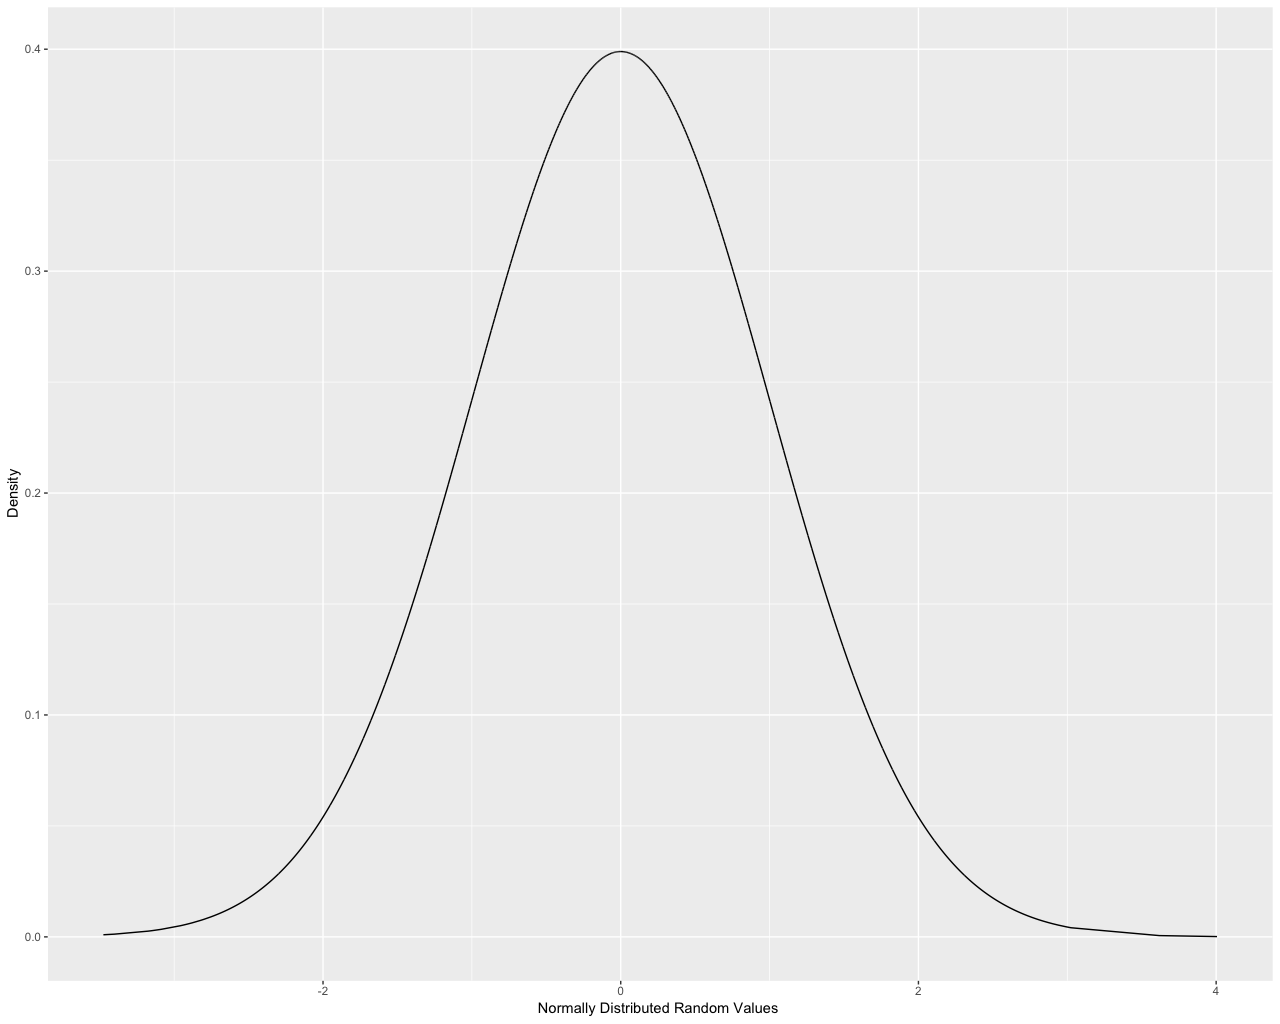
\includegraphics[width=\textwidth,height=0.75\textheight]{pic0051}\end{figure}
\end{frame}

\begin{frame}
\frametitle{Кумулативна функция на нормално разпределение}
\begin{equation}
cdf(x) = \int_{-\infty}^{a} \frac{1}{{\sigma \sqrt {2\pi } }}e^{{{ - \left( {x - \mu } \right)^2 } \mathord{\left/ {\vphantom {{ - \left( {x - \mu } \right)^2 } {2\sigma ^2 }}} \right. \kern-\nulldelimiterspace} {2\sigma ^2 }}} dx
\end{equation}
\end{frame}

\begin{frame}
\frametitle{Кумулативна функция на нормално разпределение}
\begin{figure}[]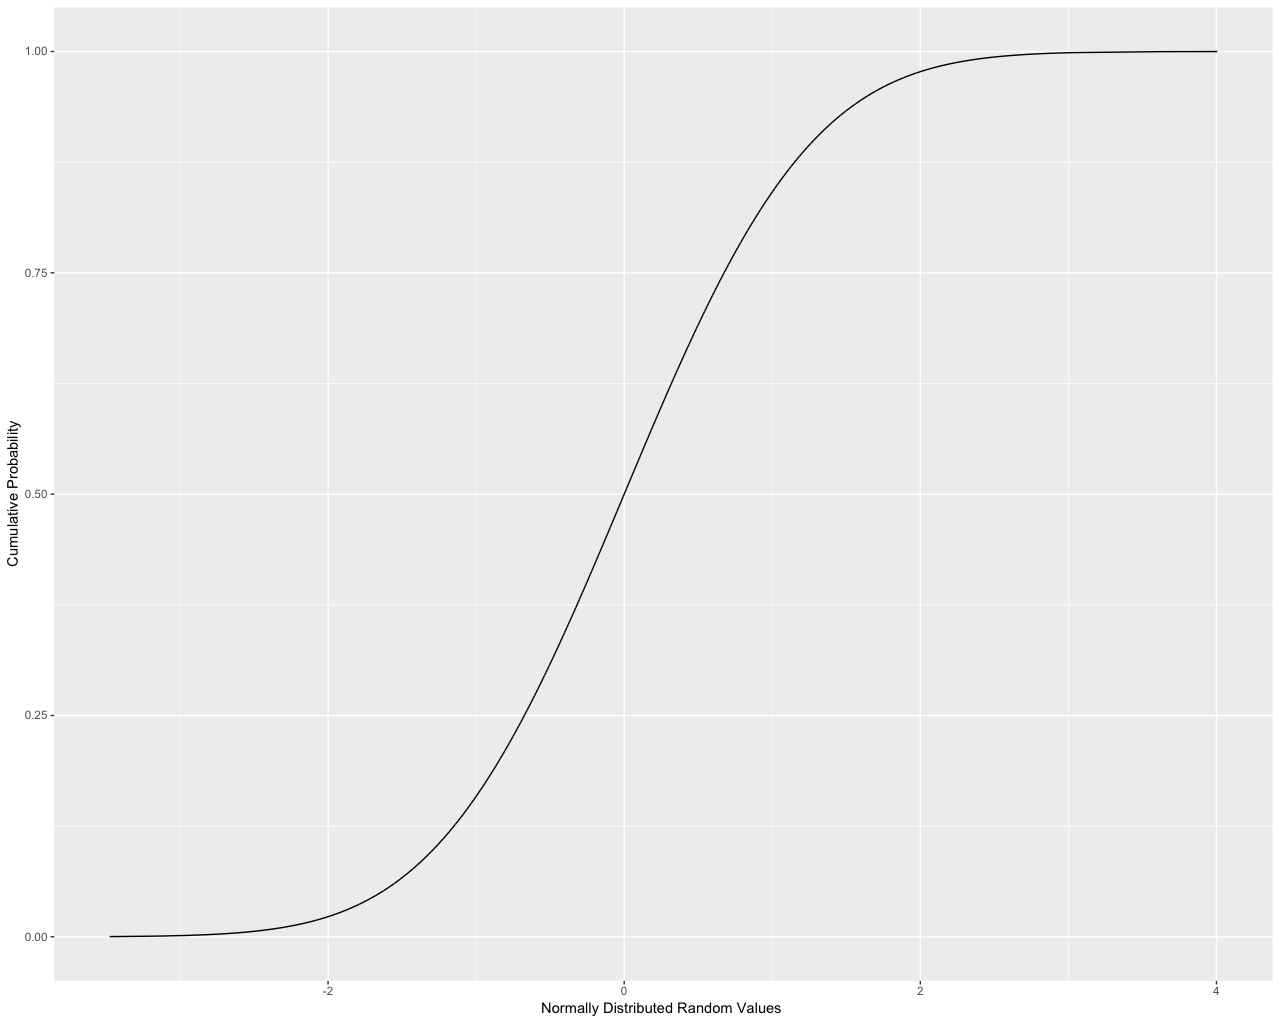
\includegraphics[width=\textwidth,height=0.75\textheight]{pic0052}\end{figure}
\end{frame}

\subsection{Биномно разпределение}

\begin{frame}
\frametitle{}
\begin{block}{}
\end{block}
\end{frame}

\section{Заключение}

\begin{frame}
\center \huge{Заключение}
\end{frame}

\subsection{Дискусия}

\begin{frame}
\frametitle{Въпроси и отговори}
\center \huge{Благодаря за вниманието!}
\end{frame}

\end{document}
